\begin{frame}
	\frametitle{Material para armado de estas slides}
	Curso de Cyrill Stashniss: \url{https://youtu.be/v-Rm9TUG9LA}

\end{frame}

\begin{frame}
    \frametitle{Mapas Grilla de Ocupación (Occupancy Grid Maps)}
    \note{información extraída de https://youtu.be/v-Rm9TUG9LA}
    
    \begin{itemize}
    \item Representación del entorno que usan en general los robots móviles.
    \item Estos tipos de mapas almacenan información sobre que áreas del mapa están ocupados (hay obstáculos) y cuales están libres (se pueden navegar). Se los puede pensar como un ``plano del lugar''.
    \item Permiten realizar planeamiento de caminos.
    \end{itemize}

    
\end{frame}

\begin{frame}
    \frametitle{Motivación: Para qué Mapear}
    \note{información extraída de https://youtu.be/v-Rm9TUG9LA}
    
    \begin{itemize}
        \item Los mapas son requeridos para la mayoría de las tareas de robótica como localización, planeamiento, etc.
        \item Tareas que requieren un entendimiento del entorno (información semántica)
        \item Aprender mapas a partir de mediciones de los sensores es una de las tareas fundamentales de las robótica móvil
    \end{itemize}
    
\end{frame}

\begin{frame}
    \frametitle{Sensores para la creación de mapas}
    \note{información extraída de https://youtu.be/v-Rm9TUG9LA}
    
    \note{Sensores exteoceptivos que nos permiten medir el entorno}
 	
   	\begin{figure}[!h]
    		\centering
    		\subfloat[]
    		{
    			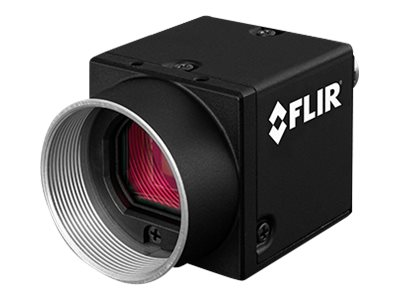
\includegraphics[width=0.15\columnwidth]{./images/flir_blackfly_s_camera.jpg}
    		}
    		\subfloat[]
    		{
    			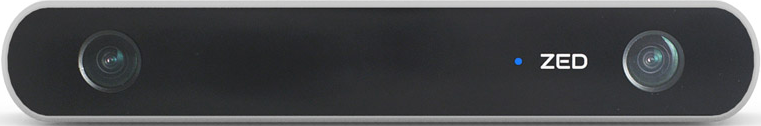
\includegraphics[width=0.2\columnwidth]{./images/stereo_camera_zed.png}
    		}
    		\subfloat[]
    		{
    			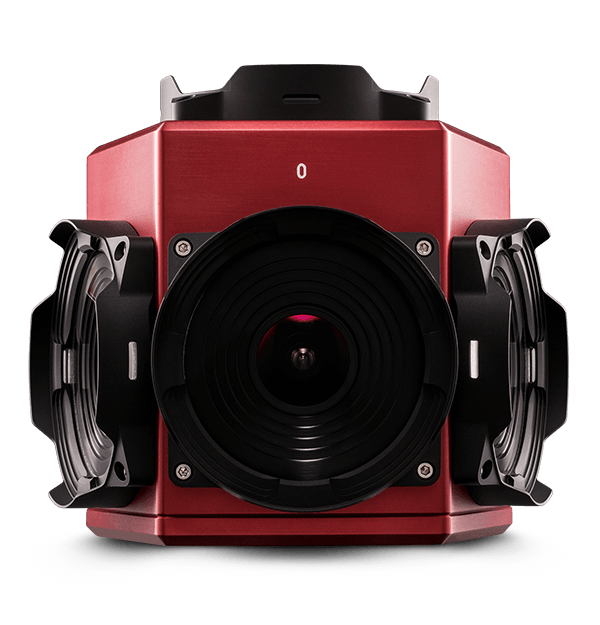
\includegraphics[width=0.1\columnwidth]{./images/ladybug5plus_360_camera.png}
    		}
    		\subfloat[]
    		{
    			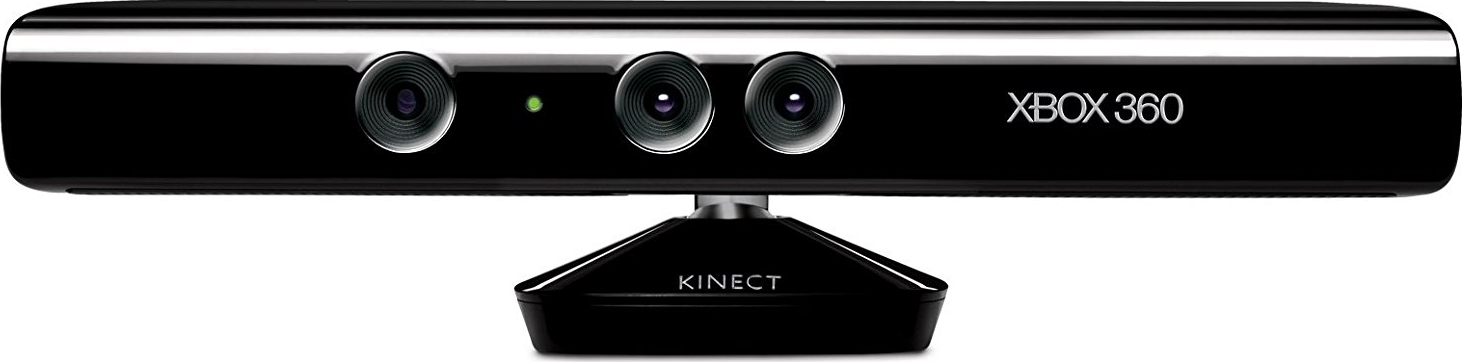
\includegraphics[width=0.2\columnwidth]{./images/structured_light_kinect.png}
    		}\\
		   	\subfloat[]
    		{
    			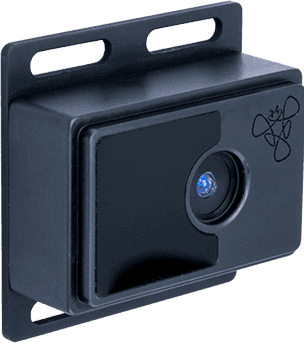
\includegraphics[width=0.15\columnwidth]{./images/terabee_time_of_flight_camera.png}
	    	}
    		\subfloat[]
    		{
    			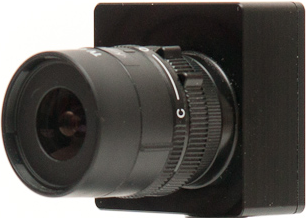
\includegraphics[width=0.2\columnwidth]{./images/event_camera_dvs128.png}
    		}
    		\subfloat[]
    		{
    			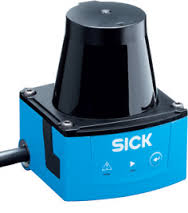
\includegraphics[width=0.15\columnwidth]{./images/lidar_sick.jpg}
    		}
	   		\subfloat[]
    		{
    			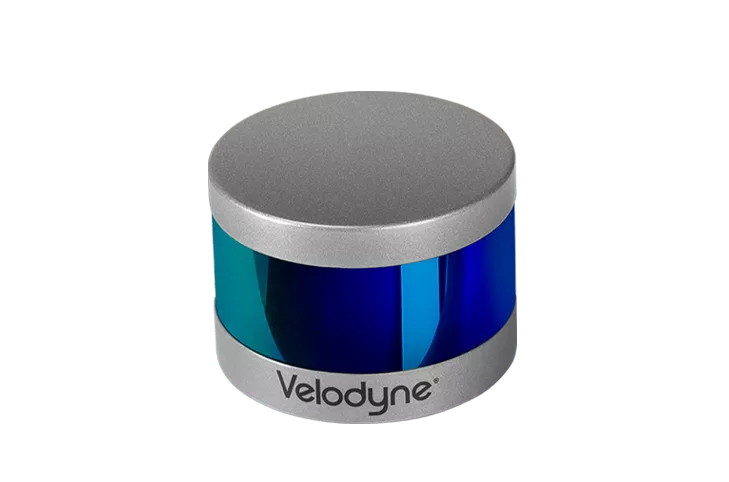
\includegraphics[width=0.15\columnwidth]{./images/velodyne_puck.png}
    		}
    	\end{figure}
    
\end{frame}

\begin{frame}
    \frametitle{Mapas Volumétricos vs Features}
    \note{información extraída de https://youtu.be/v-Rm9TUG9LA}
    
    \note{Los feature maps almacen puntos distintivos del entorno}
    
    \note{El feature map correspnode a un trabajo deEduardo Nebot en el victorial park. Los puntos amarillso son los troncos de los árboles.}
    
    \note{El feature map son útiles únicamente para localizarse pero no para navegar por el entorno ya que se desconoce que hay entre los puntos.}
    
    \note{Los mapas volumétricos 2d pueden ser vistos como un plano del piso de la habitación}
    
    \note{Los mapas volumétricos explicitamente representan las áreas libres del entorno.}
    
   	\begin{figure}[!h]
    	\centering
    	\subfloat[Mapa Volumétrico 2D]
    	{
    		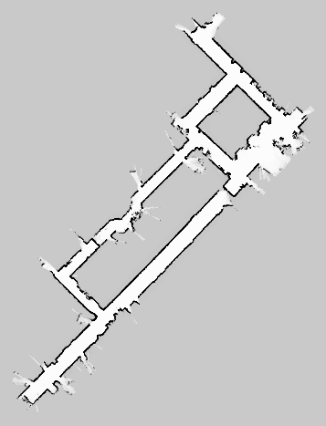
\includegraphics[width=0.23\columnwidth]{./images/volumetric_map_2d.png}
    	}
    	\subfloat[Mapa Volumétrico 3D]
    	{
    		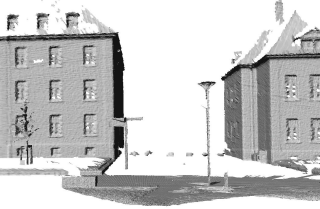
\includegraphics[width=0.3\columnwidth]{./images/volumetric_map_3d.png}
    	}
    	\subfloat[Mapa de features 2D]
    	{
    		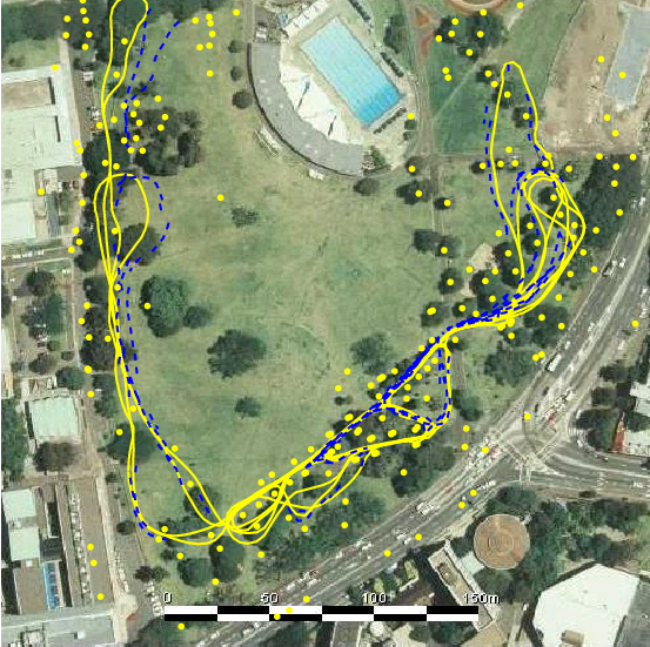
\includegraphics[width=0.3\columnwidth]{./images/feature_map_2d.png}
    	}
    \end{figure}
    
\end{frame}


\begin{frame}
    \frametitle{Mapa de Nube de puntos (Point Cloud Map)}
    \note{información extraída de https://youtu.be/v-Rm9TUG9LA}
    
    
   	\begin{figure}
    	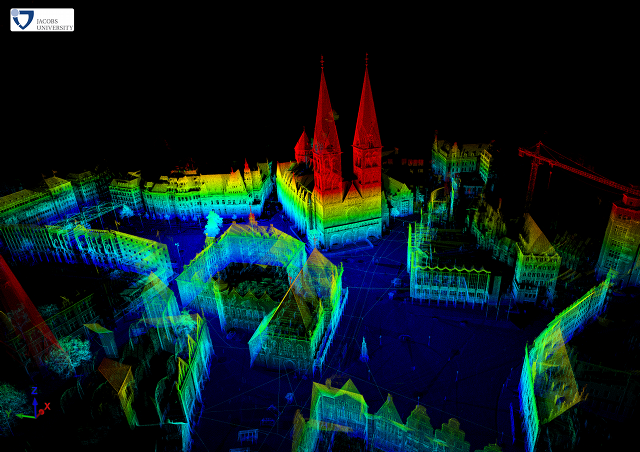
\includegraphics[width=0.6\columnwidth]{./images/point_cloud_map_bremen_city.png}
    \end{figure}
    
\end{frame}


\begin{frame}
	\frametitle{Mapa Semántico (Semantic Map)}
	\note{información extraída de https://youtu.be/v-Rm9TUG9LA}
	
   	\begin{figure}
    	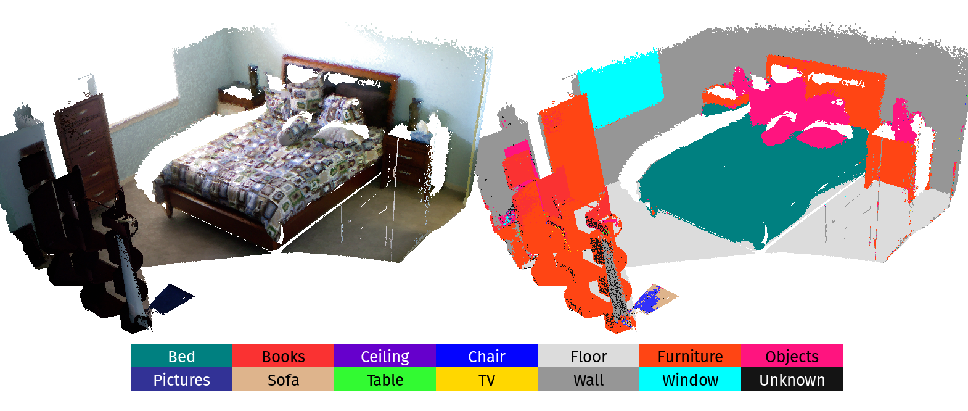
\includegraphics[width=0.6\columnwidth]{./images/semantic_map_semanticfusion.png}
	\end{figure}
	
	
\end{frame}


\begin{frame}
    \frametitle{Recontrucción de mapas}
    \note{información extraída de https://youtu.be/v-Rm9TUG9LA}
    
\end{frame}

\begin{frame}
    \frametitle{Mapas de Grilla}
    \note{información extraída de https://youtu.be/v-Rm9TUG9LA}
    
    
\end{frame}

\begin{frame}
    \frametitle{Ejemplo de Mapa de Grilla}
    \note{información extraída de https://youtu.be/v-Rm9TUG9LA}
    
    
\end{frame}

\begin{frame}
    \frametitle{Mapas de Grilla}
    \note{información extraída de https://youtu.be/v-Rm9TUG9LA}
    
    
\end{frame}

\begin{frame}
    \frametitle{Mapas de Grilla}
    \note{información extraída de https://youtu.be/v-Rm9TUG9LA}
    
    
\end{frame}

\begin{frame}
    \frametitle{Mapas de Grilla}
    \note{información extraída de https://youtu.be/v-Rm9TUG9LA}
    
    
\end{frame}

\begin{frame}
    \frametitle{Mapas de Grilla}
    \note{información extraída de https://youtu.be/v-Rm9TUG9LA}
    
    
\end{frame}

\begin{frame}
    \frametitle{Mapas de Grilla}
    \note{información extraída de https://youtu.be/v-Rm9TUG9LA}
    
    
\end{frame}

\begin{frame}
    \frametitle{Mapas de Grilla}
    \note{información extraída de https://youtu.be/v-Rm9TUG9LA}
    
    
\end{frame}
